\documentclass[aspectratio=169]{beamer} % O parâmetro aspectratio com valar 16:9 deixa o slide em widescreen

\usepackage[brazil]{babel}
\usepackage[utf8]{inputenc}
\usepackage[T1]{fontenc}

\usetheme{Madrid}
\setbeamertemplate{navigation symbols}{}

\title[Educação em Tecnologias Digitais]{Educação em Tecnologias Digitais}

\author[Diego S. C. Nascimento]{Diego Silveira Costa Nascimento}

\institute[IFRN]{
Instituto Federal de Educação, Ciência e Tecnologia do Rio Grande do Norte\\
diego.nascimento@ifrn.edu.br
}

\date[\today]{\today}

\begin{document}

\begin{frame}[plain]
	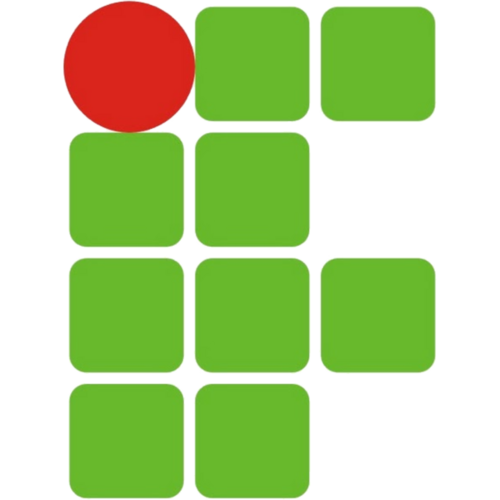
\includegraphics[scale=0.2]{img/IFRN}
	\titlepage
\end{frame}

\logo{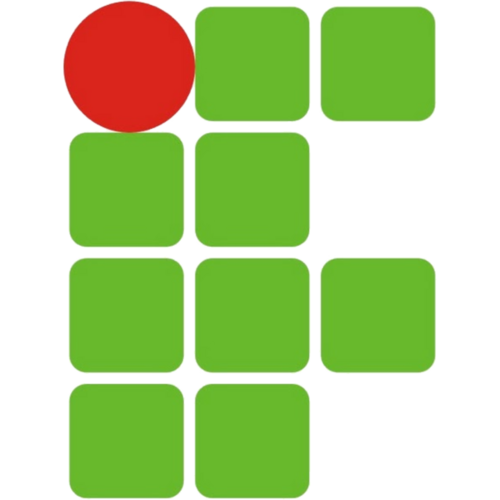
\includegraphics[scale=0.1]{img/IFRN}}

\begin{frame}
	\frametitle{Ementa do Curso}
  	\tableofcontents
\end{frame}

\AtBeginSection[]{
	\begin{frame}
		\frametitle{Ementa}
		\tableofcontents[currentsection]
	\end{frame}
}

\section{Sistemas Operacionais}

\begin{frame}
	\frametitle{Sistema Operacional}
	
	\begin{block}{Definição}
		É um programa ou um conjunto de programas cuja função é gerenciar os recursos do sistema, fornecendo uma interface entre o computador e o usuário.	
	\end{block}\vfill
	
	\begin{exampleblock}{Exemplos}
		\begin{itemize}
			\item Windows;
			\item Linux;
			\item MacOS;
			\item Chrome OS; 
			\item Android; e
			\item IOS.
		\end{itemize}
	\end{exampleblock}
\end{frame}

\begin{frame}
	\frametitle{Principais Funções}
	
	\begin{itemize}
		\item Gerenciamento de processos;
		\item Gerenciamento de memória;
		\item Gerenciamento de recursos;
		\item Entrada e saída de dados; e
		\item Sistema de arquivos.
	\end{itemize}
\end{frame}

\begin{frame}
	\frametitle{Windows}
	
	\begin{itemize}
		\item Teve a primeira versão lançada em 1985; e
		\item É uma família de sistemas operacionais comercializados e vendidos pela Microsoft.
	\end{itemize}\vfill
	
	\begin{center}
		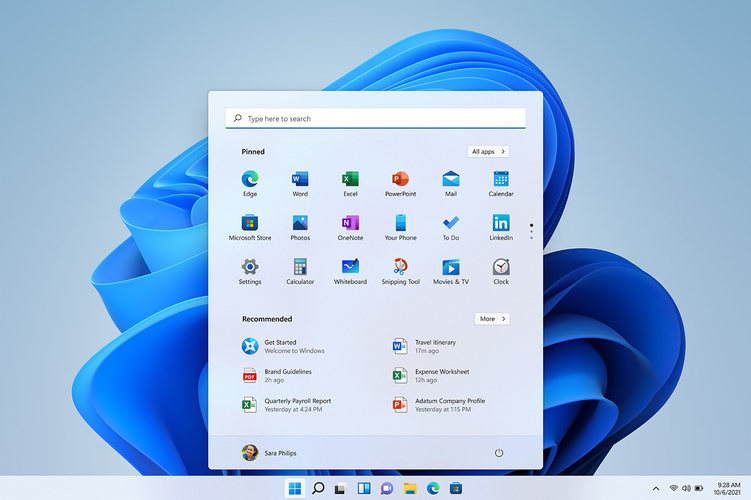
\includegraphics[scale=1]{img/windows11}
	\end{center}
\end{frame}

\begin{frame}
	\frametitle{Linux}
	
	\begin{itemize}
		\item Foi desenvolvido pelo programador finlandês Linus Torvalds, inspirado no sistema Minix; 
		\item Teve a primeira versão lançada em 1991; e
		\item O código-fonte está disponível sob a licença GPL (versão 2) para que qualquer pessoa o possa utilizar, estudar, modificar e distribuir livremente.
	\end{itemize}\vfill
	
	\begin{center}
		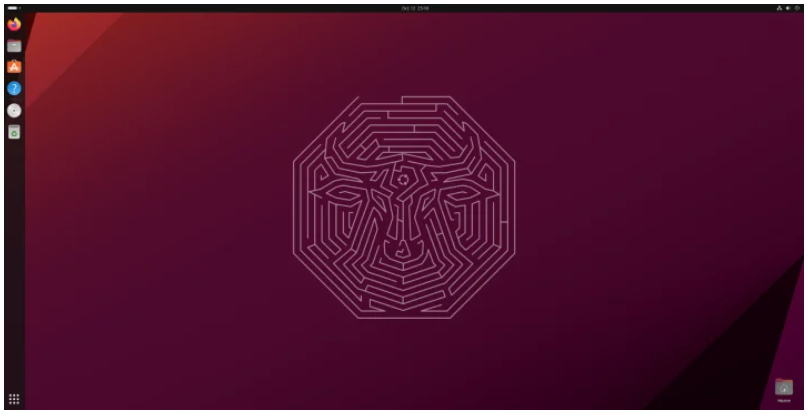
\includegraphics[scale=0.4]{img/ubuntu2310}
	\end{center}
\end{frame}

\begin{frame}
	\frametitle{MacOS}
	
	\begin{itemize}
		\item É um sistema operacional proprietário desenvolvido e distribuído pela Apple;
		\item Teve a primeira versão lançada em 1984.
	\end{itemize}\vfill
	
	\begin{center}
		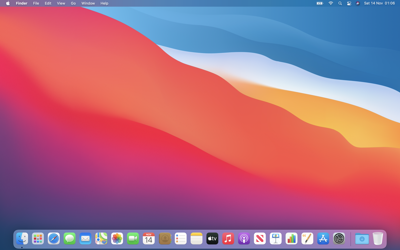
\includegraphics[scale=0.45]{img/macosbig}
	\end{center}
\end{frame}

\begin{frame}
	\frametitle{Chrome OS}
	
	\begin{itemize}
		\item É um sistema operacional desenvolvido pelo Google;
		\item Teve a primeira versão lançada em 2010; e
		\item É baseado no núcleo do Linux. 
	\end{itemize}\vfill
	
	\begin{center}
		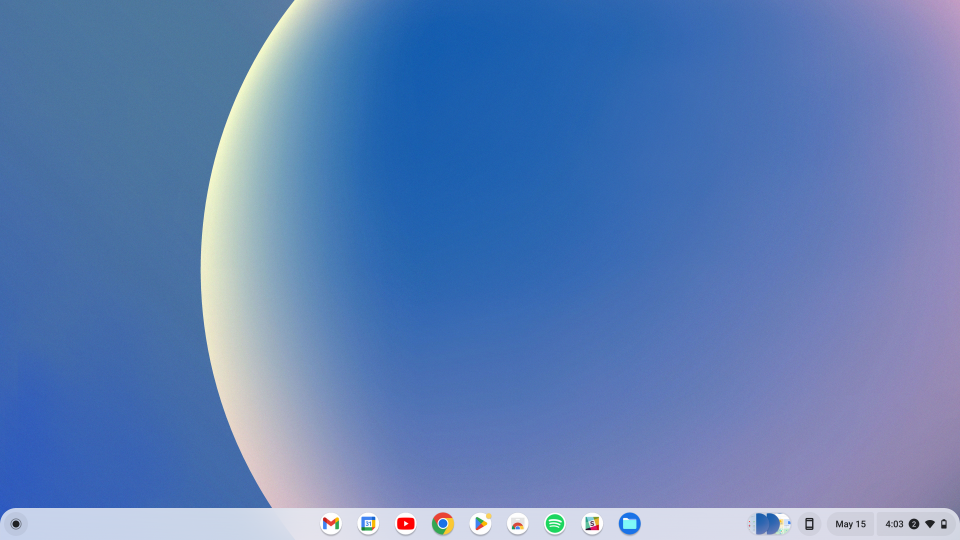
\includegraphics[scale=0.2]{img/chromeos}
	\end{center}
\end{frame}

\begin{frame}
	\frametitle{Android}
	
	\begin{itemize}
		\item Desenvolvido por um consórcio de desenvolvedores conhecido como Open Handset Alliance, sendo o principal colaborador o Google;
		\item Projetado principalmente para dispositivos móveis;
		\item Teve a primeira versão lançada em 2008; e
		\item É baseado no núcleo do Linux. 
	\end{itemize}\vfill
	
	\begin{center}
		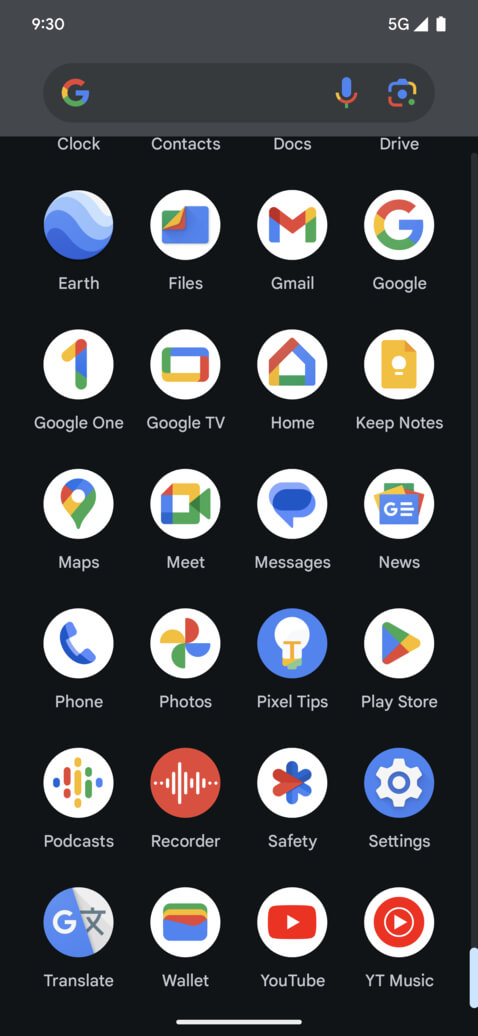
\includegraphics[scale=0.13]{img/android}
	\end{center}
\end{frame}

\begin{frame}
	\frametitle{IOS}
	
	\begin{itemize}
		\item Desenvolvido pela Apple;
		\item Projetado para dispositivos móveis; e
		\item Teve a primeira versão lançada em 2007.
	\end{itemize}\vfill
	
	\begin{center}
		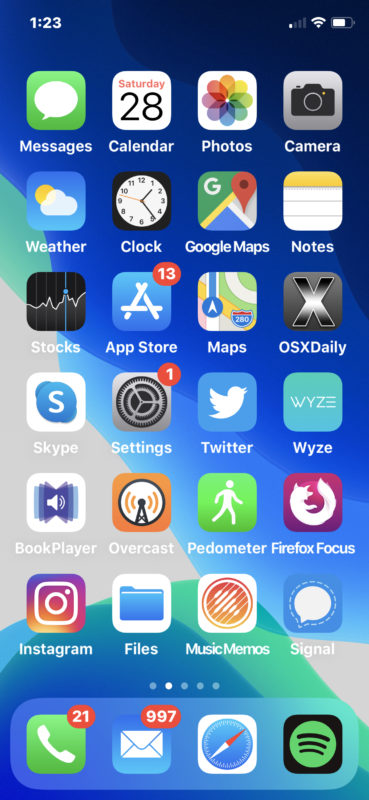
\includegraphics[scale=0.15]{img/ios}
	\end{center}
\end{frame}

\begin{frame}
	\frametitle{Usando um Sistema Operacional}
	
	\begin{itemize}
		\item Área de trabalho;
		\item Menu de programas;
		\item Barra de tarefas;
		\item Lixeira.
	\end{itemize}
\end{frame}

\begin{frame}
	\frametitle{Janela}
	
	\begin{itemize}
		\item Barra de título;
		\item Menu;
		\item Minimizar;
		\item Maximizar/Restaurar; e
		\item Fechar.
	\end{itemize}
\end{frame}

\begin{frame}
	\frametitle{Gerenciador de Arquivos}
	
	\begin{block}{Definição}
		 É um programa de computador usado para criar e organizar diretórios e arquivos em sistemas operacionais.
	\end{block}
	
	\begin{center}
		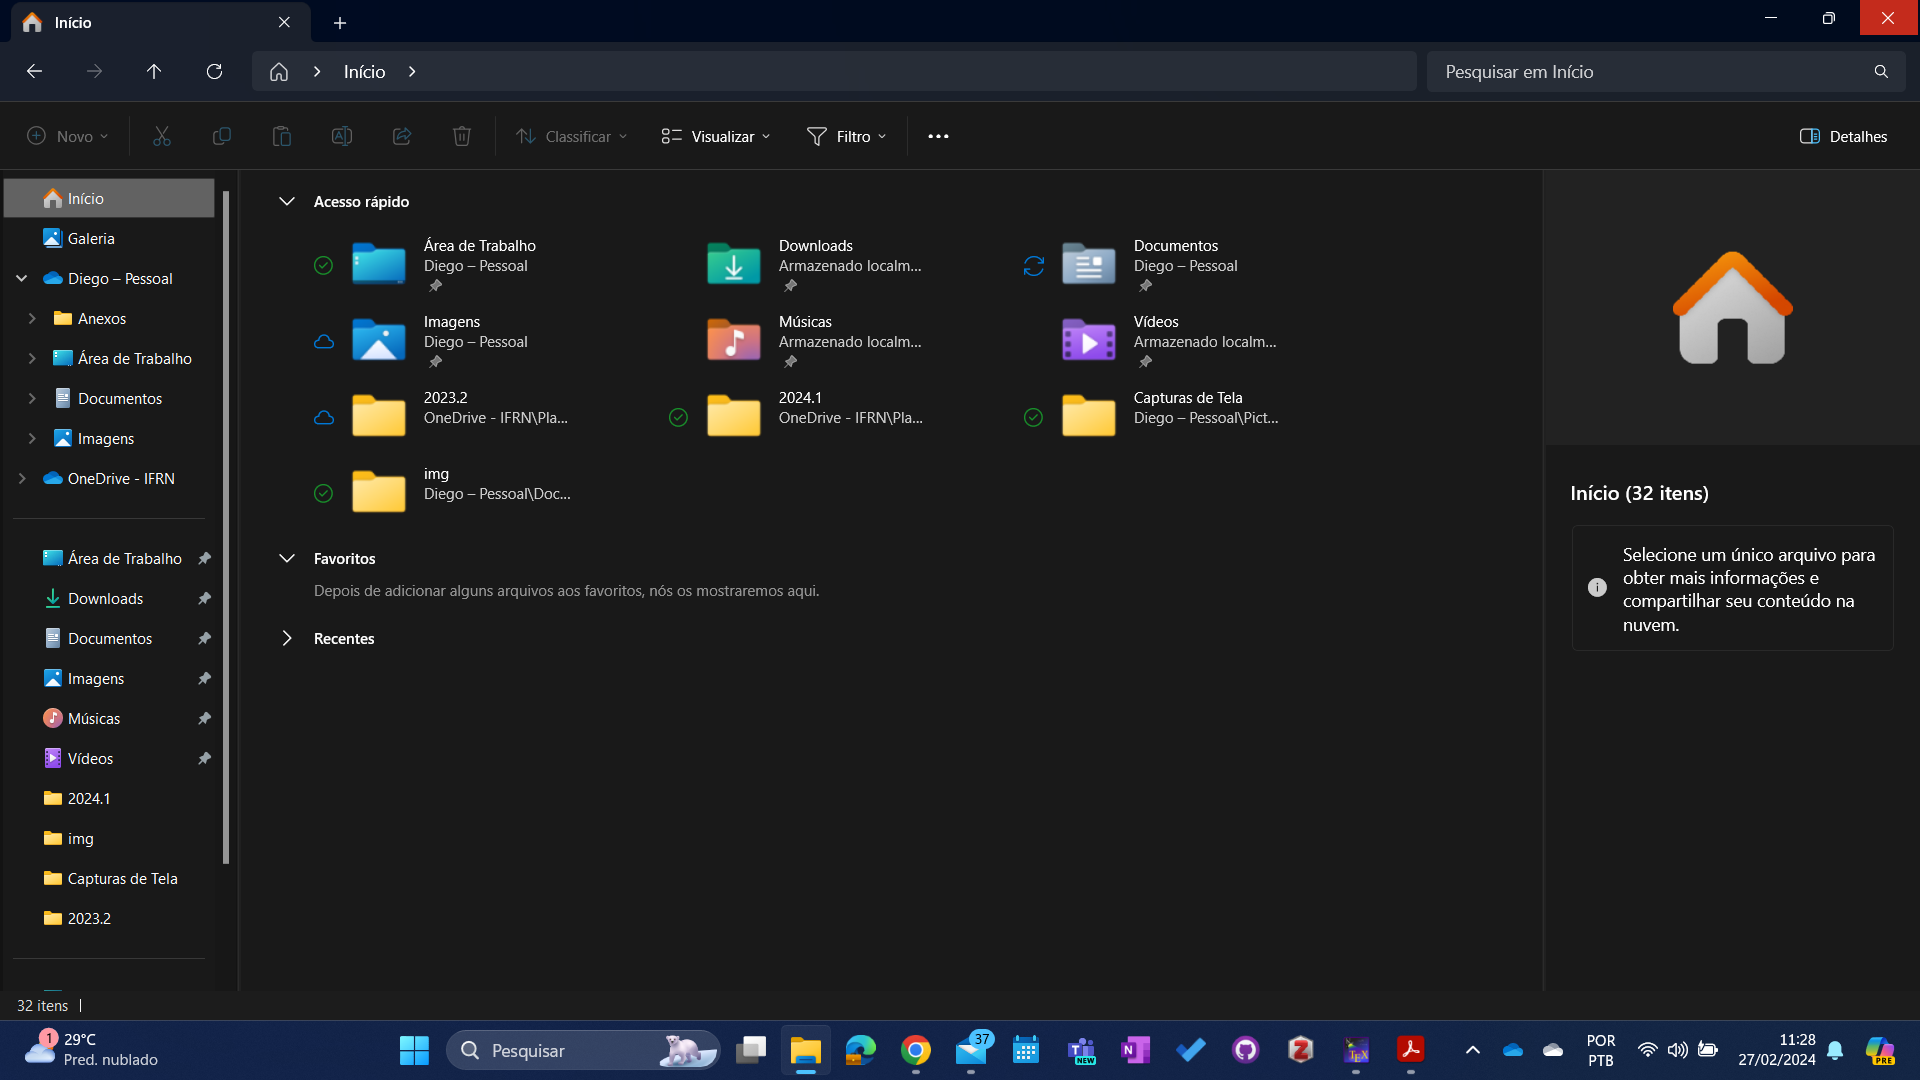
\includegraphics[scale=0.1]{img/explorador-de-arquivos}
	\end{center}
\end{frame}

\begin{frame}
	\frametitle{Configura\c cões do Sistema}
	
	\begin{itemize}
		\item Aparência; e
		\item Idioma;
		\item Contas da internet;
		\item Impressora;
		\item Teclado;
		\item Mouse;
		\item Atualiza\c cões do sistema; e
		\item Instala\c cão de programas.
	\end{itemize}
\end{frame}

\begin{frame}
	\frametitle{Encerramento do Sistema}
	
	\begin{itemize}
		\item Suspender;
		\item Reiniciar; e
		\item Desligar.
	\end{itemize}
\end{frame}

\begin{frame}
	\frametitle{Softwares Utilitários}
	
	\begin{block}{Defini\c cão}
		São software projetados para fornecer funcionalidades adicionais e recursos que não são encontrados nos sistemas operacionais padrão.
	\end{block}\vfill
	
	\begin{exampleblock}{Exemplos}
		\begin{itemize}
			\item Compactadores;
			\item Antivírus;
			\item Bacakup; e
			\item Desfragmentador de disco.
		\end{itemize}
	\end{exampleblock}
\end{frame}

\begin{frame}
	\frametitle{Compacta\c cão de Arquivos}
	
	\begin{block}{Defini\c cão}
		São softwares especializados em gerar uma representação mais eficiente de vários arquivos dentro de um único arquivo de modo que ocupem menos espaço na mídia de armazenamento.
	\end{block} \vfill
	
	\begin{exampleblock}{Exemplos}
		\begin{itemize}
			\item 7-Zip;
			\item WinZip; e
			\item WinRAR.
		\end{itemize}
	\end{exampleblock}
\end{frame}

\begin{frame}
	\frametitle{Antivírus}
	
	\begin{block}{Defini\c cão}
		É é um programa utilizado para prevenir, detectar e eliminar malware e vírus.
	\end{block}\vfill

	\begin{exampleblock}{Programas}
		\begin{itemize}
			\item McAfee;
			\item Microsoft Defender;
			\item Avast;
			\item AVG.
		\end{itemize}
	\end{exampleblock}
\end{frame}

\begin{frame}
	\frametitle{Backup}
	
	\begin{block}{Defini\c cão}
		É um termo utilizado para uma atividade que consiste em realizar cópias de segurança de dados digitais de um dispositivo com o intuito de recuperá-los em caso de perdas acidentais ou falhas no sistema em que os arquivos estão armazenados.
	\end{block}
\end{frame}

\begin{frame}
	\frametitle{Desfragmentador de Arquivos}
	
	\begin{block}{Defini\c cão}
		É uma ferramenta que permite analisar o desfragmentar unidades de disco, tornando o computador mais rápido, eficiente e ganhando velocidade.
	\end{block}\vfill
	
	\begin{center}
		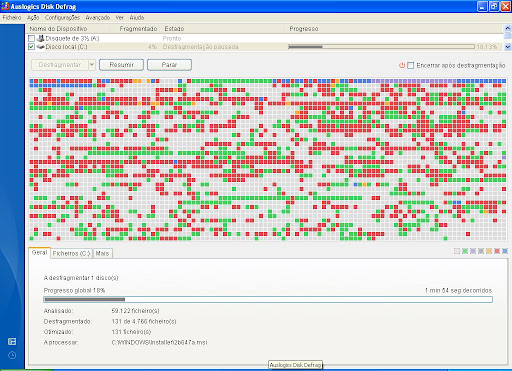
\includegraphics[scale=0.4]{img/desfragmentador}
	\end{center}
\end{frame}

\section{Internet}

\section{Inteligência Artificial na Educação}

\section{Editor de Texto}

\section{Editor de Apresentação}

\section{Editor de Planilha Eletrônica}

\end{document}